\documentclass[a4paper, 12pt]{article}

\usepackage[utf8]{inputenc}
\usepackage{graphicx}
\usepackage{amsmath}
\usepackage{amssymb}
\usepackage{siunitx}
\usepackage{float}
\usepackage{placeins}
\usepackage{xstring}
\usepackage{geometry}
\usepackage{enumitem}
\usepackage{listings}
\usepackage{color}
\usepackage{subcaption}
%\usepackage[defaultlines=4,all]{nowidow}
\usepackage[hidelinks]{hyperref}
\usepackage{cleveref}


\geometry{tmargin=2.5cm, bmargin=3cm}

% Geen geïndenteerde paragrafen, da's maar lelijk.
\setlength{\parindent}{0pt}
% Wel spatie tussen paragrafen please.
\setlength{\parskip}{1em}

% Exponential notation in '\num{}'w/ Ex instead of *10^x
\sisetup{output-exponent-marker=\ensuremath{\mathrm{E}}}

% Necessary to make space->underscore substitution work. 
\usepackage[T1]{fontenc}
% Command that typesets variables in fixed width font, and with spaces automatically replaced by underscores.
% May need to be prepended by a '\protect' in a \caption.
\newcommand{\varr}[1]{\texttt{\StrSubstitute{#1}{ }{\_\allowbreak}}}

% For identifying individual datapoints -- i.e. cars.
\newcommand{\car}[3]{``#1 \textit{#2} #3''}

\newcommand{\wide}[1]{\makebox[\textwidth][c]{#1}%
}

% For figures accross the page -- wider than the text width
\newcommand{\widefig}[1]{\wide{\includegraphics[width=0.9\paperwidth]{#1}}}

\newcommand{\widesubfig}[2]{\wide{
  \centering
  \begin{subfigure}[b]{0.65\textwidth}
    #1
  \end{subfigure}
  \begin{subfigure}[b]{0.65\textwidth}
    #2
  \end{subfigure}
  }
}

\newcommand{\widetwofigs}[2]{\wide{
  \centering
  \begin{minipage}[t]{0.62\textwidth}
  #1
  \end{minipage}
  \hspace{1em}
  \begin{minipage}[t]{0.62\textwidth}
  #2
  \end{minipage}
 }
}

\newcommand{\sectionref}[1]{section ``\nameref{#1}''}

% Shortcut
\newcommand{\n}[1]{\num{#1}}

\begin{document}


\begin{titlepage}
    \newpage
    \thispagestyle{empty}
    \frenchspacing
    \hspace{-0.2cm}
    
\includegraphics[height=4.2cm]{fig/sedes}
    \hspace{0.2cm}
    \rule{0.5pt}{4.2cm}
    \hspace{0.2cm}
    \begin{minipage}[b]{8cm}
        \Large{Katholieke\newline Universiteit\newline Leuven}\smallskip\newline
%         \large{}\smallskip\newline
%         \textbf{Departement Wiskunde}\newline
%         Afdeling Statistiek
    \end{minipage}
    \hspace{\stretch{1}}
    \vspace*{3.2cm}\vfill
    \begin{center}
        \begin{minipage}[t]{\textwidth}
            \begin{center}
            	\LARGE{\rm{Statistische Modellen \& Data-analyse}}\\[5mm]
                \LARGE{\rm{\textbf{Practicum 2}}}
            \end{center}
        \end{minipage}
    \end{center}
    \vfill
    \hfill\makebox[8.5cm][l]{%
        \vbox to 7cm{\vfill\noindent
        	\large{{\rm\textbf{Tomas Fiers}}\\[2mm]
                   {\rm Juni 2017}}
        }
    }
\end{titlepage}


\section{Linear regression}

The complete dataset of 1500 cars was split into a 1000-car training set and a 500-car test set. We continue this analysis with the training set.

\subsection*{Exploratory analysis \& outlier removal}
\label{sec:RD_outlier_removal}

We search for outliers by calculating, for each data point, its statistical distance to the multivariate distribution -- using robust estimates for the center and the covariance matrix. Specifically, the Minimum Covariance Determinant estimator \cite{mcd} was used, approximated by the \texttt{Fast MCD} algorithm \cite{fastmcd}. \Cref{fig:RD_outliers} shows the resulting robust distances.

\begin{figure}%[h]
  \widefig{fig/multivar_outlier_all}
  \vspace{1mm} \newline
  \widefig{fig/multivar_outlier_zoom}
  \caption{Robust distance-to-center of each car in the training set.}
  \label{fig:RD_outliers}
\end{figure}

Three strong outliers are found:
\begin{itemize}[topsep=0pt,itemsep=0pt]
  \item the \car{Volkswagen}{Jetta (from NOV 06 Wk 45 >)}{1.4 TSI (170 PS) Sport} with an abnormal \varr{noise level} of 0.3;
  \item the \car{Vauxhall}{Signum MY2008}{3.0CDTi V6 24v with 16/17/18" wheel} with an abnormal \varr{nox emissions} value of 237000;
  \item the \car{MG Rover Group}{Streetwise}{1.8} without any individually abnormal variables.
\end{itemize}
Note that this third outlier would not have been found had we only looked at univariate (or even bivariate) distributions of the data.

The found strong outliers are removed from the training set.


\begin{figure}%[H]
  \widefig{fig/pairs.pdf}
  \caption{Uni- and bivariate sample distributions (after the strongest robust distance-outliers have been removed).}
  \label{fig:pairs}
\end{figure}

\Cref{fig:pairs} shows the uni- and bivariate distributions in the data set. Note the very strong correlations between \varr{urban metric}, \varr{extra urban metric}, \varr{combined metric}, and \varr{co2} -- and to a lesser extend \varr{engine capacity}. This is in accordance with their meanings: cars with larger engine volumes consume more liters of fuel (all three \varr{ metrics} measure fuel consumption), and every liter of fuel corresponds to a fixed amount of $\mathrm{CO_2}$. These strong pairwise correlations point to the problem of multicollinearity in the data set. We explore this more formally further on.

We also note that for the variable \varr{noise level}, a large subset of cars take on discrete values. (There are also cars with \varr{noise level}s in between). This discrete character would negatively impact a cluster analysis, as the clusters would tend to form around the disrete values; while other variables would have disproportionately less impact on the clustering. However, we decide this will probably not impact the subsequent regression and classification tasks too much, so we keep this variable, for now.

Additionally, we note that none of the continuous variables seem to be univariate normally distributed (further on we do numeric normality tests, and normal QQ plots have been checked). Rather, they are positively skewed, with heavy right tails.

Finally, note the multimodality of \varr{engine capacity} and \varr{nox emissions}, and the fact that \varr{fuel type} tends to split the other variables into groups -- see e.g. \varr{Diesel} versus \varr{Hybrid} or \varr{Petrol} for \varr{nox emissions}.


\subsection*{Model construction}

We will construct a general linear model to predict the \varr{co2} variable. The predictor variables to include in the model will be selected via bidirectional stepwise regression. The Akaike Information Criterion (AIC) is used to compare models. The least squares estimator will always be used to estimate the coefficients $\boldsymbol{\beta}$ for a candidate model. The categorical variables \varr{euro standard}, \varr{transmission type}, and \varr{fuel type} are expanded into indicator variables (e.g. \varr{fuel type Petrol}, taking on either a 0 or a 1).

\paragraph{Predictor variable transformations}
\label{sec:var_transform}\leavevmode\\
The AIC assumes the residuals to be normally distributed. As they are an affine transformation of the predictor variables, the predictor variables need to be normally distributed as well. Thus, before starting the stepwise variable selection procedure, we find a Box-Cox power transformation \cite{boxcox} for all continuous predictor variables that maximises their normality in the maximum likelihood sense. The thusly found exponents $\lambda$ are listed in \cref{table:predictorvar_transform}, along with the $p$-values for the Shapiro-Wilk test of normality before and after the transformation. Note that, except for \varr{noise level}, the normality of each variable greatly increases after the transformation. This was confirmed using normal QQ plots of the variables. We apply the maximum likelihood transformation to all continuous predictor variables, except for \varr{noise level} (as its maximum likelihood exponent falls outside the usual range, and its normality does not significantly improve after transformation).

\begin{table}
\centering
\begin{tabular}{r|r|c|c}
Variable & $\lambda_{ML}$ & $p_{before}$ & $p_{after}$ \\
\hline
\varr{engine capacity}    & \num{-0.65} & \num{4E-33} & \num{2E-12} \\
\varr{urban metric}       & \num{-0.06} & \num{2E-23} & \num{0.164} \\
\varr{extra urban metric} & \num{-0.64} & \num{3E-22} & \num{0.002} \\
\varr{combined metric}    & \num{-0.37} & \num{3E-23} & \num{0.011} \\
\varr{noise level}        & \num{ 7.11} & \num{2E-14} & \num{3E-12} \\
%\varr{co2}                & \num{-0.18} & \num{5E-21} & \num{0.067} \\
\varr{co emissions}       & \num{ 0.29} & \num{7E-26} & \num{0.093} \\
\varr{nox emissions}      & \num{ 0.04} & \num{1E-35} & \num{1E-12}
\end{tabular}

\caption{Maximum likelihood transformation exponents $\lambda$, and $p$-values for the Shapiro-Wilk test of normality before and after transformation, for each possible continuous predictor variable.}
\label{table:predictorvar_transform}
\end{table}

\paragraph{Response variable transformation}
\label{sec:responsevar_transfrom}\leavevmode\\
We now create a first linear model (via stepwise AIC regression starting from a model containing all predictor variables). \Cref{fig:pre-bc-response} shows the residuals of the resulting model. The strong (nonlinear) correlation between the predicted \varr{co2} values and the residuals prompts us to transform the response variable. The optimal Box-Cox power transformation of the response variable \cite{boxcox} is found for $\lambda = -0.3$ (see \cref{fig:lambda_ml}). We create a new linear model with the transformed response variable.

\begin{figure}
  \widetwofigs
  {
    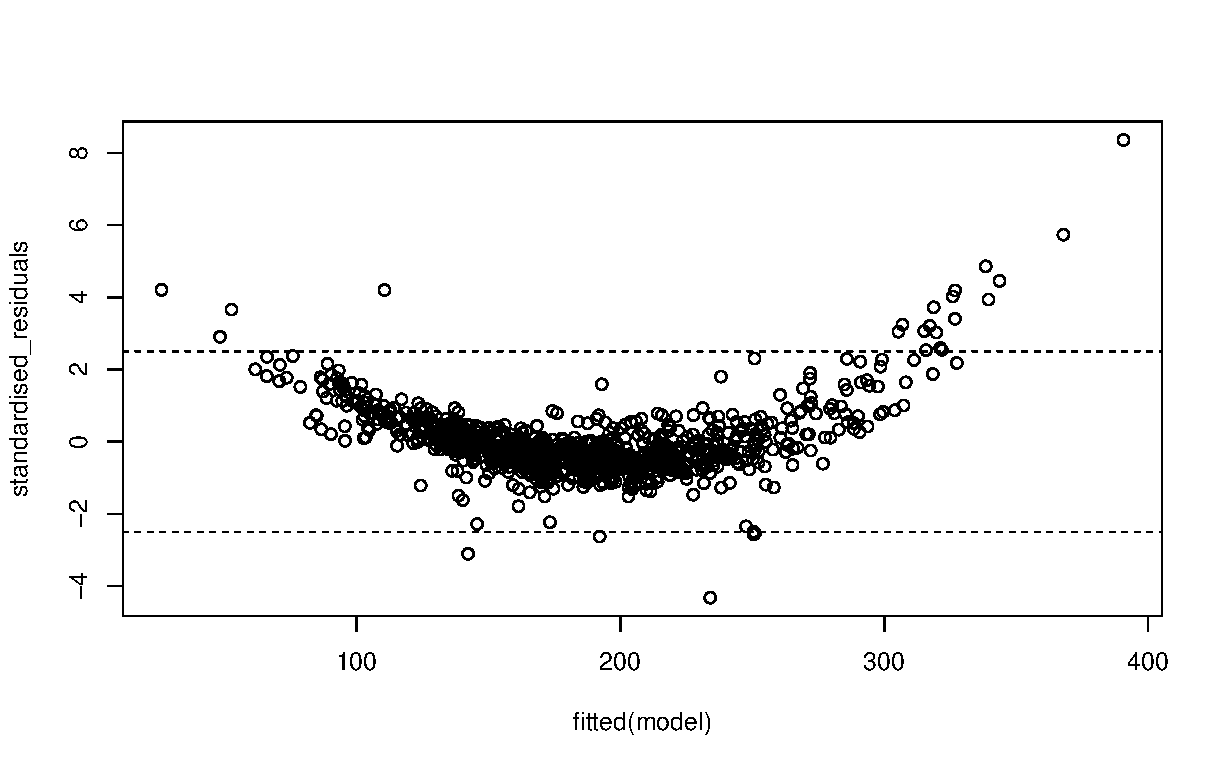
\includegraphics[width=\textwidth, trim={0 3mm 0 2cm}, clip]
    {fig/pre-bc-response_pre-removal_fitted-stdres}
    \caption{Standardised residuals of the linear model versus fitted values, before the response variable has been transformed.}
    \label{fig:pre-bc-response}
  }
  {
    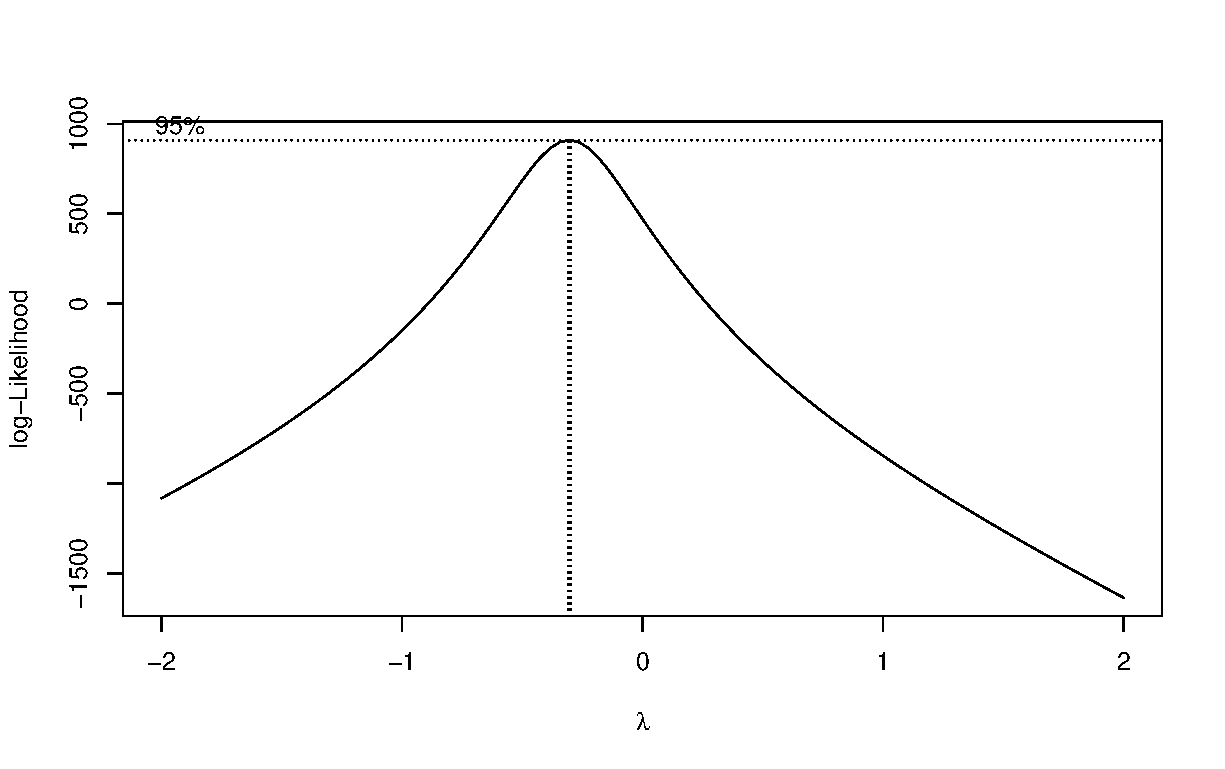
\includegraphics[width=\textwidth, trim={0 3mm 0 2cm}, clip]
    {fig/pre-bc-response_pre-removal_lambda-ml}
    \caption{Log-likelihood of $\lambda$ for the Box-Cox transformation of the response variable.}
    \label{fig:lambda_ml}
  }
\end{figure}

\paragraph{Removal of residual outliers}\leavevmode\\
The residuals of the model with transformed response variable are shown in \cref{fig:post-bc-response_pre-removal}. We find three strong vertical outliers. They are:
\begin{itemize}[topsep=0pt,itemsep=0pt]
  \item the \car{Volkswagen}{LT 35 Kombi MWB - LWB}{2.8 (158 PS) TDI Axle Ratio 3.727};
  \item the \car{Honda}{Insight, Model Year 2012}{1.3 IMA HS, HS-T, HX};
  \item and the \car{Renault}{New M\'egane Hatchback}{2.0 dCi 160 FAP}.
\end{itemize}
(These cars do not have higher robust distances than other cars (as in \cref{fig:RD_outliers}); they can however be spotted as outliers when the Mahalonobis distance is considered). These three additional outliers are removed from the training set. We note that removing these outliers has no effect on the maximum-likelihood $\lambda$ of the Box-Cox transformation of the response variable.

\begin{figure}
  \captionsetup[subfigure]{skip=0pt}
  \caption{Standardised residuals of the linear model versus fitted values, after the response variable has been transformed.}
  \widesubfig
  {
    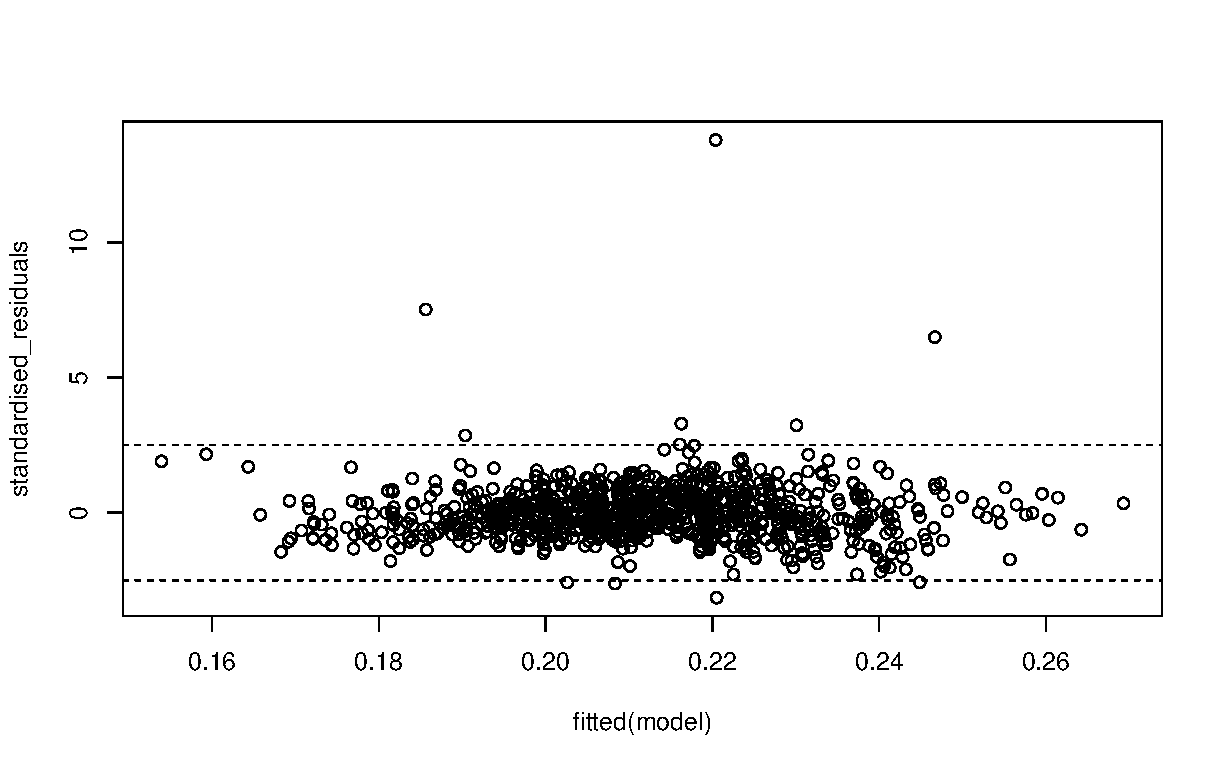
\includegraphics[width=\textwidth, trim={0 3mm 0 2cm}, clip]
    {fig/post-bc-response_pre-removal_fitted-stdres}
    \caption{Before removal of vertical outliers.}
    \label{fig:post-bc-response_pre-removal}
  }{
    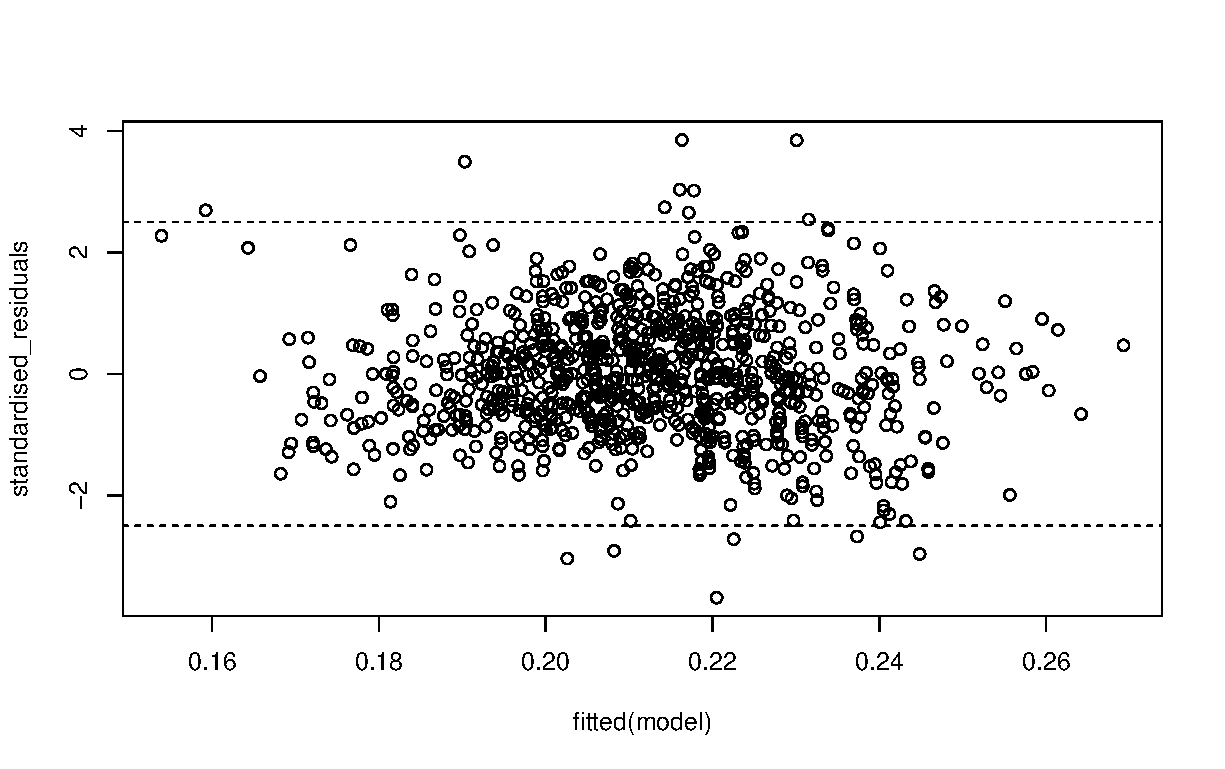
\includegraphics[width=\textwidth, trim={0 3mm 0 2cm}, clip]
    {fig/post-bc-response_post-removal_fitted-stdres}
    \caption{After removal of vertical outliers.}
    \label{fig:post-bc-response_post-removal}
  }
\end{figure}

\paragraph{Variable selection \& final model}\leavevmode\\
With optimal input and output transformations and the strongest outliers removed, we can now construct our final model, by selecting an appropriate subset of predictor variables. As already mentioned, bidirectional stepwise AIC regression is used. The procedure is started both from a model containing all predictor variables, and from an empty model containing only a constant term. Both procedures converge to the same model. The included variables, along with estimates for their coefficient and an analysis of variance (ANOVA), are shown in \cref{table:lm}. The variables that are not included, are \varr{noise level} and \varr{transmission type Manual}. We find a final $R^2$ value of 0.9987, an adjusted $R^2$ value of 0.9987, and a mean squared error $\hat{\sigma}^2$ of $4.750\times 10^{-7}$. The standardised residuals are shown in \cref{fig:post-bc-response_post-removal}.

\begin{table}
\centering
\hspace{-1cm}
\wide{\newcommand{\al}[1]{\multicolumn{1}{l|}{\n{#1}}} % Align a number left
\newcommand{\NA}{--} % not available
\newcommand{\cs}[1]{\multicolumn{1}{c|}{#1}}  % center - single border
\newcommand{\cd}[1]{\multicolumn{1}{c||}{#1}} % center - double border
\newcommand{\cn}[1]{\multicolumn{1}{c}{#1}}   % center - no border
\newcommand{\rs}[1]{\multicolumn{1}{r|}{#1}}  % right  - single border

\begin{tabular}{r|r||r|r|r|r||r|r|r}
Predictor variable $j$           &
\cd{$\lambda_j$}                 &
\cs{$\hat{\beta_j}$}             &
\cs{$\mathrm{s}(\hat{\beta_j})$} &
\cs{$t$}                         &
\cd{$p$}                         &
\cs{SS}                          &
\cs{$F$}                         &
\cn{$Pr(>F)$}                    \\
\hline
(Intercept)               & \cd{\NA}    & \n{ 5.3E-01} & \n{2.8E-02}& \n{ 18.9} & \n{ 3E-68} & \al{45.6}  & \n{95972309} & \n{<2E-16} \\
\varr{engine capacity}    & \num{-0.65} & \n{-9.3E-02} & \n{1.8E-02}& \n{ -5.1} & \n{ 5E-07} & \n{0.1663} & \n{  350125} & \n{<2E-16} \\
\varr{urban metric}       & \num{-0.06} & \n{-2.2E-02} & \n{1.2E-03}& \n{-18.4} & \n{ 3E-65} & \n{0.1771} & \n{  372852} & \n{<2E-16} \\
\varr{extra urban metric} & \num{-0.64} & \n{-5.5E-02} & \n{3.7E-03}& \n{-14.7} & \n{ 2E-44} & \n{0.0032} & \n{    6710} & \n{<2E-16} \\
\varr{combined metric}    & \num{-0.37} & \n{-5.4E-02} & \n{4.5E-03}& \n{-12.0} & \n{ 7E-31} & \n{0.0001} & \n{     229} & \n{<2E-16} \\
\varr{co emissions}       & \num{ 0.29} & \n{-2.6E-05} & \n{7.6E-06}& \n{ -3.5} & \n{ 6E-04} & \n{0.0010} & \n{    2149} & \n{<2E-16} \\
\varr{nox emissions}      & \num{ 0.04} & \n{ 7.2E-05} & \n{3.7E-05}& \n{  2.0} & \n{ 5E-02} & \n{0.0058} & \n{   12130} & \n{<2E-16} \\
\varr{euro standard 4}    & \cd{\NA}    & \n{ 3.7E-04} & \n{7.0E-05}& \n{  5.2} & \n{ 2E-07} & \n{0.0002} & \n{     506} & \n{<2E-16} \\
\varr{euro standard 5}    & \cd{\NA}    & \n{ 1.4E-03} & \n{7.9E-05}& \n{ 18.0} & \n{ 5E-63} & \n{0.0002} & \n{     391} & \n{<2E-16} \\
\varr{euro standard 6}    & \cd{\NA}    & \n{ 1.0E-03} & \n{1.6E-04}& \n{  6.0} & \n{ 2E-09} & \n{0.0002} & \n{     388} & \n{<2E-16} \\
\varr{fuel type Hybrid}   & \cd{\NA}    & \n{ 7.5E-03} & \n{1.7E-04}& \n{ 44.0} & \n{2E-234} & \n{0.0002} & \n{     390} & \n{<2E-16} \\
\varr{fuel type Petrol}   & \cd{\NA}    & \n{ 7.5E-03} & \n{1.4E-04}& \n{ 54.7} & \n{2E-300} & \n{0.0014} & \n{    2993} & \n{<2E-16} \\
(Residuals)               & \cd{\NA}    & \cs{\NA}     & \cs{\NA}   & \cs{\NA}  & \cd{\NA}   & \n{0.0005} & \rs{\NA}     & \cn{\NA}   \\
\end{tabular}
}
\caption{Coefficients and ANOVA of the final general linear model. $\lambda_j$'s taken from \cref{table:predictorvar_transform}. Note that both the predictor variables and the response variable are transformed non-linearly. That is why some coefficients may seem counterintuitive at first -- e.g. a negative slope for \protect\varr{engine capacity} with respect to \protect\varr{co2}.}
\label{table:lm}
\end{table}


\subsection*{Discussion}

\paragraph{Performance on the test set}\leavevmode\\
As we have a proper test set at our disposal, we can check whether our model generalises well. It does. The mean absolute relative error (defined as $\frac{1}{n-p}\sum_{i=1}^{n}{\left| \frac{\hat{y_i}-y_i}{y_i}\right|}$) on the test set is $2.9\times 10^{-3}$, demonstrating excellent predictive power -- the $\mathrm{CO_2}$ emissions of a car can be predicted with an error of on average only 0.3\%. The mean squared error on the test set is $8.00\times 10^{-7}$, indicating that our previous estimate $\hat{\sigma}^2 = 4.75\times 10^{-7}$ was a decent one.

\paragraph{Gauss-Markov conditions}\leavevmode\\
We check whether our final model satisfies the Gauss-Markov conditions. The first condition, that the errors have expectation zero, is satisfied by construction. The other two conditions -- that the errors have equal variance and are uncorrelated -- cannot be proven to be satisfied, but we can check whether some necessary conditions seem to be satisfied. All residual plots -- residuals versus their index, residuals versus the fitted values, and residuals versus each of the independent variables -- need to be free of correlation. No curvature, funnel or trend should be visible. All named residual plots have been checked -- both for the training set as well as for the test set. (One such plot can be seen in \cref{fig:post-bc-response_post-removal}). No visible correlations were found, supporting the hypothesis that the Gauss-Markov conditions are reasonably well satisfied.

\paragraph*{Normality}\leavevmode\\
Most steps in the construction and analysis of our model assume the errors to be normally distributed (e.g. the Box-Cox transformation of the response variable, the AIC, and the statistics for the coefficients and the ANOVA in \cref{table:lm}). Based on the normal QQ plots of \cref{fig:qq_plots}, we pose that the errors are roughly normally distributed, but with tails that are too heavy. (The $p$ values for the Shapiro-Wilk test of normality are \n{0.01} and \n{<2E-16} for the training and test set, respectively). This less-than-ideal normality does not seem to be a problem during model construction. It does have the result however that the statistics and $p$-values in \cref{table:lm} need to be taken with a grain of salt.

\begin{figure}
  \caption{Normal QQ plots of linear model residuals}
  \widesubfig
  {
    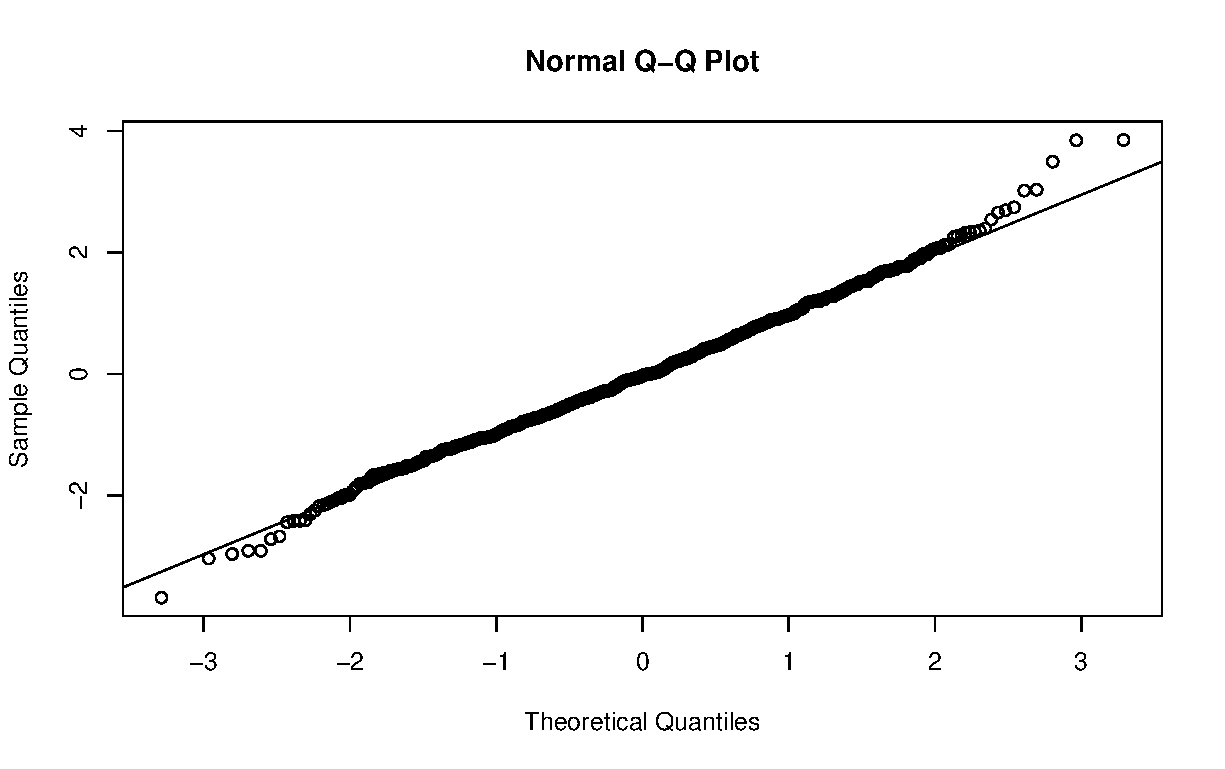
\includegraphics[width=\textwidth, trim={0 0 0 2cm}, clip]
    {fig/post-bc-response_post-removal_qq}
    \caption{Training set standardised residuals}
  }{
    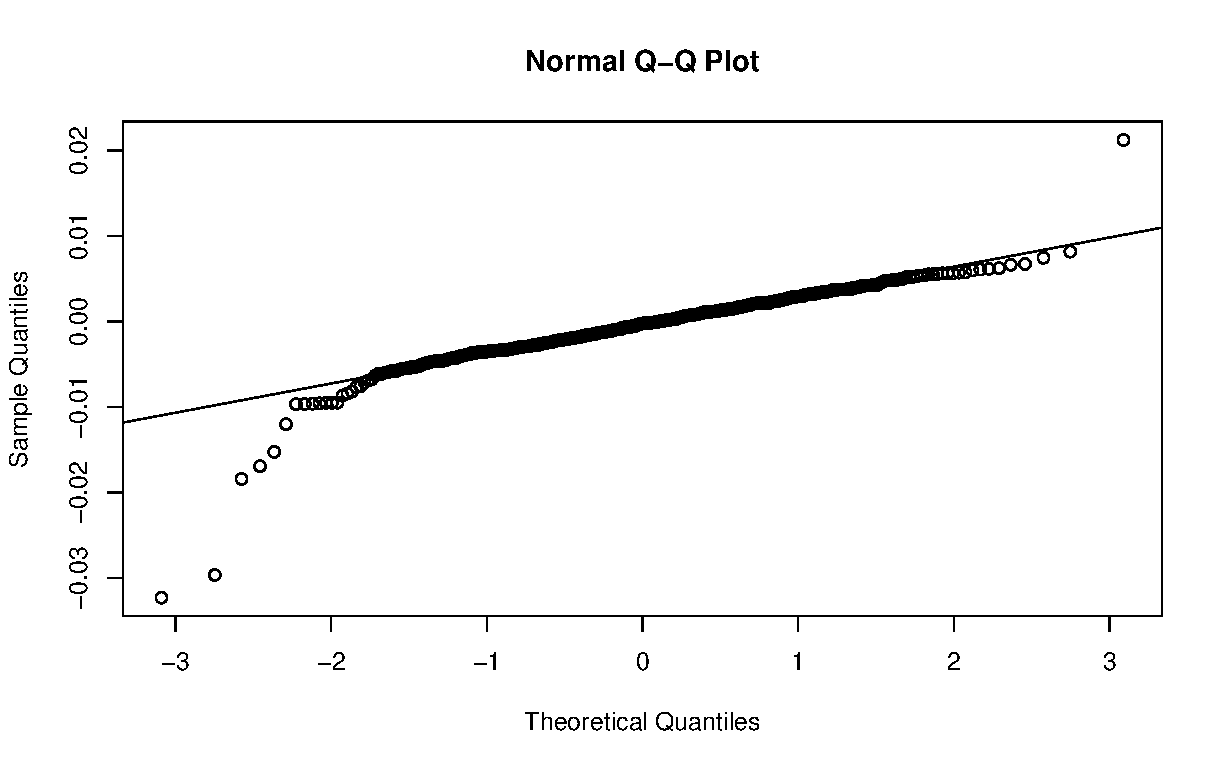
\includegraphics[width=\textwidth, trim={0 0 0 2cmm}, clip]
    {fig/test_set_qq}
    \caption{Test set residuals}
  }
  \label{fig:qq_plots}
\end{figure}

\paragraph*{Multicollinearity}\leavevmode\\
In the exploratory analysis, we noted the strong pairwise correlations between \varr{urban metric}, \varr{extra urban metric}, \varr{combined metric}, and \varr{co2}. This points to the problem of multicollinearity. Indeed, when we perform more formal tests, strong evidence is found for multicollinearity in the data: the variance inflation factors (VIF) of the mentioned variables are all larger than 100, and the mean VIF is 456, significantly larger than 1. The condition number $ \sqrt{\lambda_{max} / \lambda_{min}} = 129 $ is greater than 30 (where $\lambda$ are the eigenvalues of the corrrelation matrix of the data). In the preceding linear regression, we have ignored this multicollinearity. In the following exercise however, we will use a biased regression method with smaller variance as a remedy.

\section{Classification}
blablie

\begin{figure}
\centering
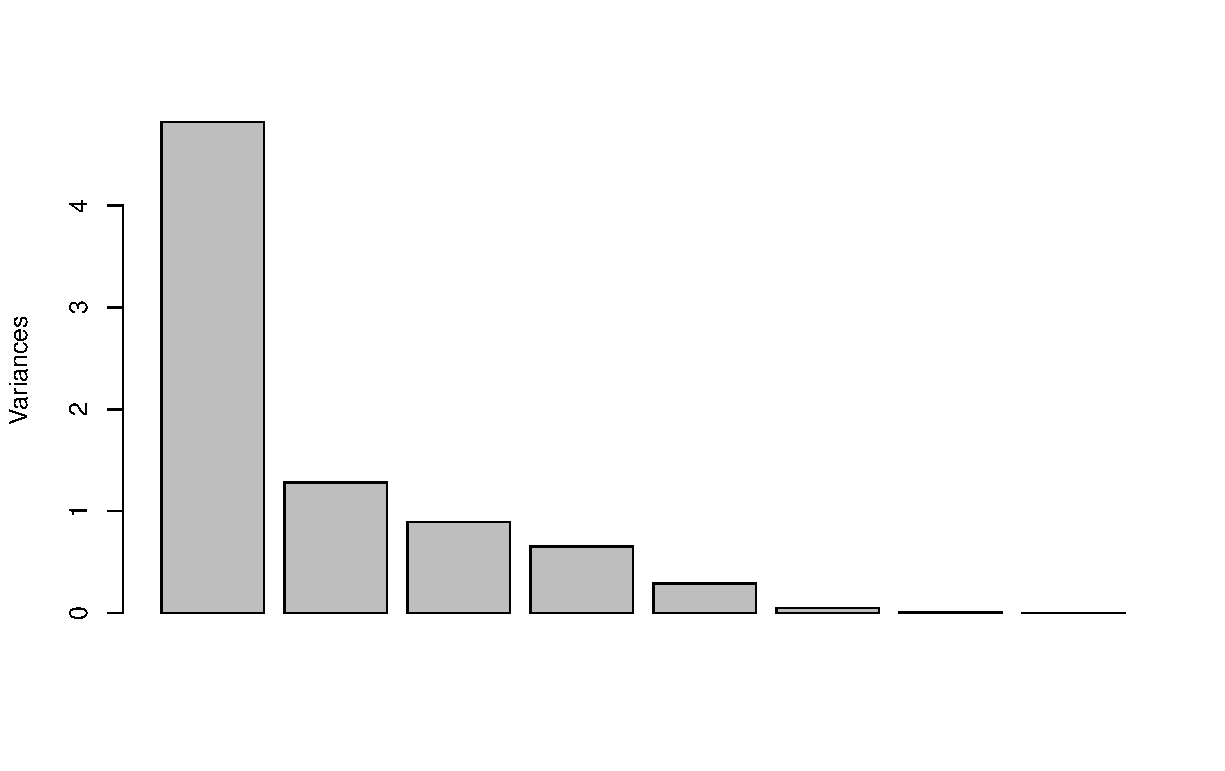
\includegraphics[width=0.7\linewidth]{fig/screeplot}
\caption{}
\label{fig:screeplot}
\end{figure}
\begin{figure}
\centering
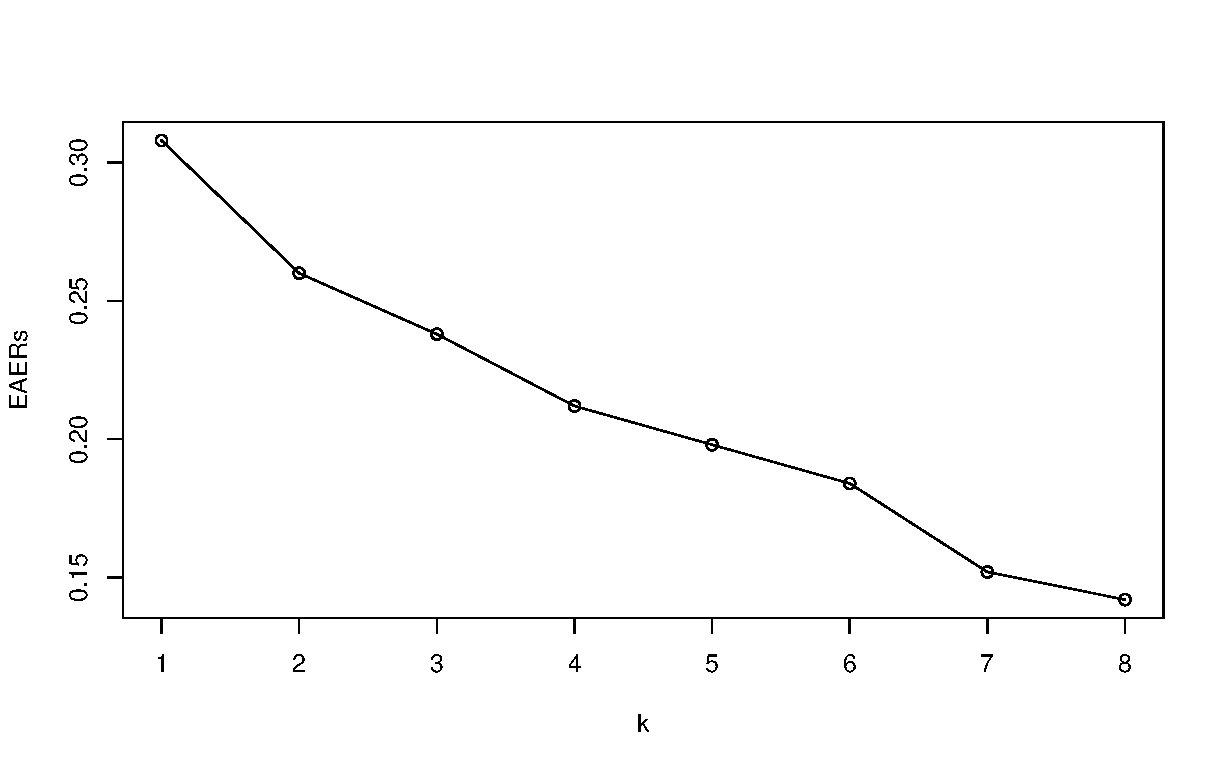
\includegraphics[width=0.7\linewidth]{fig/k_search}
\caption{}
\label{fig:ksearch}
\end{figure}

\begin{table}
\centering
%\hspace{-1cm}
\wide{\begin{tabular}{r|r||r|r|r|r||r|r|r}
Predictor variable $j$  &  $ \hat{\beta}^+ $  & PC1 & PC2 & PC3 & PC4 & PC5 & PC6 \\
\hline
(Intercept)                     & \num{ 1.70} \\
\varr{engine capacity}          & \num{ 1.07} & \num{0.355} & \num{ 0.192} & \num{-0.371} & \num{-0.220} & \num{ 0.806} & \num{-0.014} \\
\varr{urban metric}             & \num{-1.70} & \num{0.447} & \num{-0.021} & \num{-0.040} & \num{ 0.042} & \num{-0.222} & \num{-0.638} \\
\varr{extra urban metric}       & \num{ 1.16} & \num{0.444} & \num{-0.003} & \num{-0.065} & \num{ 0.073} & \num{-0.201} & \num{ 0.764} \\
\varr{combined metric}          & \num{-0.51} & \num{0.451} & \num{-0.016} & \num{-0.052} & \num{ 0.054} & \num{-0.214} & \num{-0.059} \\
\varr{noise level}              & \num{ 0.01} & \num{0.182} & \num{ 0.337} & \num{ 0.757} & \num{-0.527} & \num{ 0.044} & \num{ 0.020} \\
\varr{co2}                      & \num{-1.01} & \num{0.447} & \num{ 0.092} & \num{-0.052} & \num{ 0.112} & \num{-0.184} & \num{-0.061} \\
\varr{co emissions}             & \num{-0.17} & \num{0.190} & \num{-0.557} & \num{ 0.508} & \num{ 0.474} & \num{ 0.412} & \num{-0.001} \\
\varr{nox emissions}            & \num{-4.53} & \num{0.065} & \num{ 0.728} & \num{ 0.140} & \num{ 0.653} & \num{ 0.094} & \num{-0.016} \\
\varr{transmission type Manual} & \num{-0.59} \\
\varr{fuel type Hybrid}         & \num{-4.99} \\
\varr{fuel type Petrol}         & \num{-4.44} \\
\end{tabular}
}
\caption{}
\label{table:lrm}
\end{table}

\begin{figure}
\centering
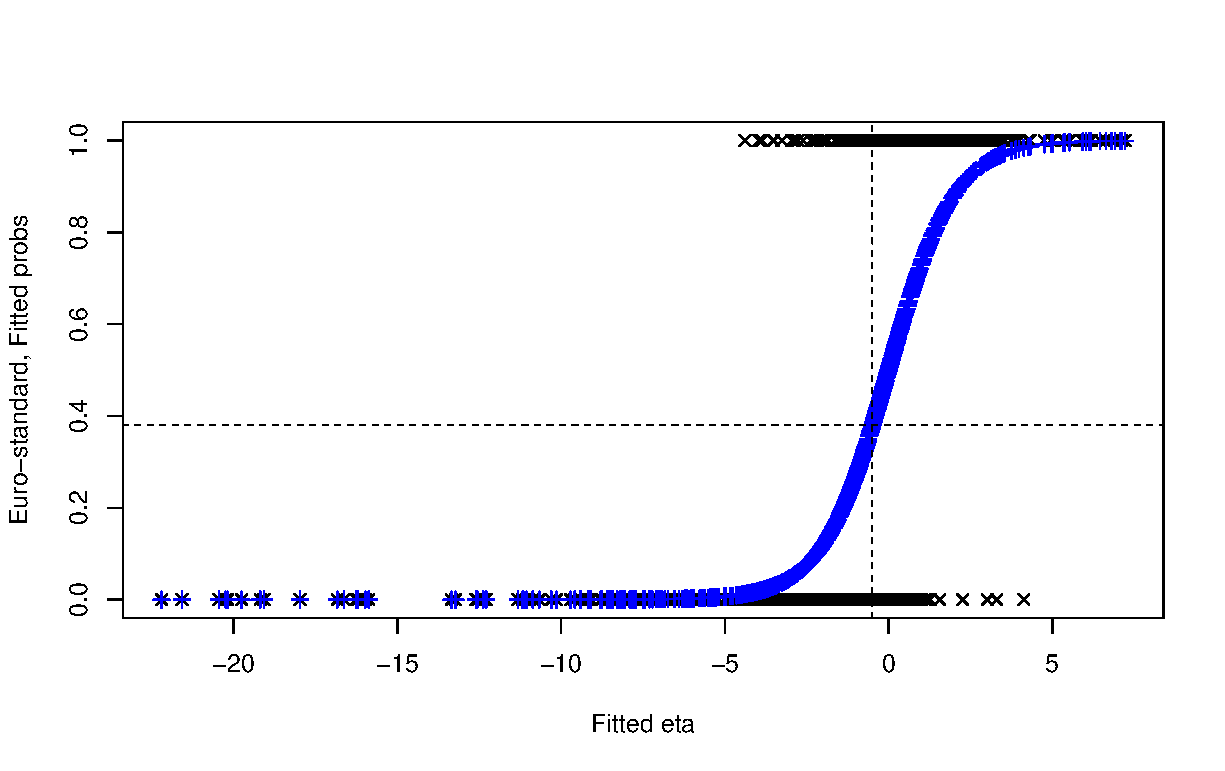
\includegraphics[width=0.7\linewidth]{fig/logistic_fit}
\caption{}
\label{fig:logisticfit}
\end{figure}
\begin{figure}
\centering
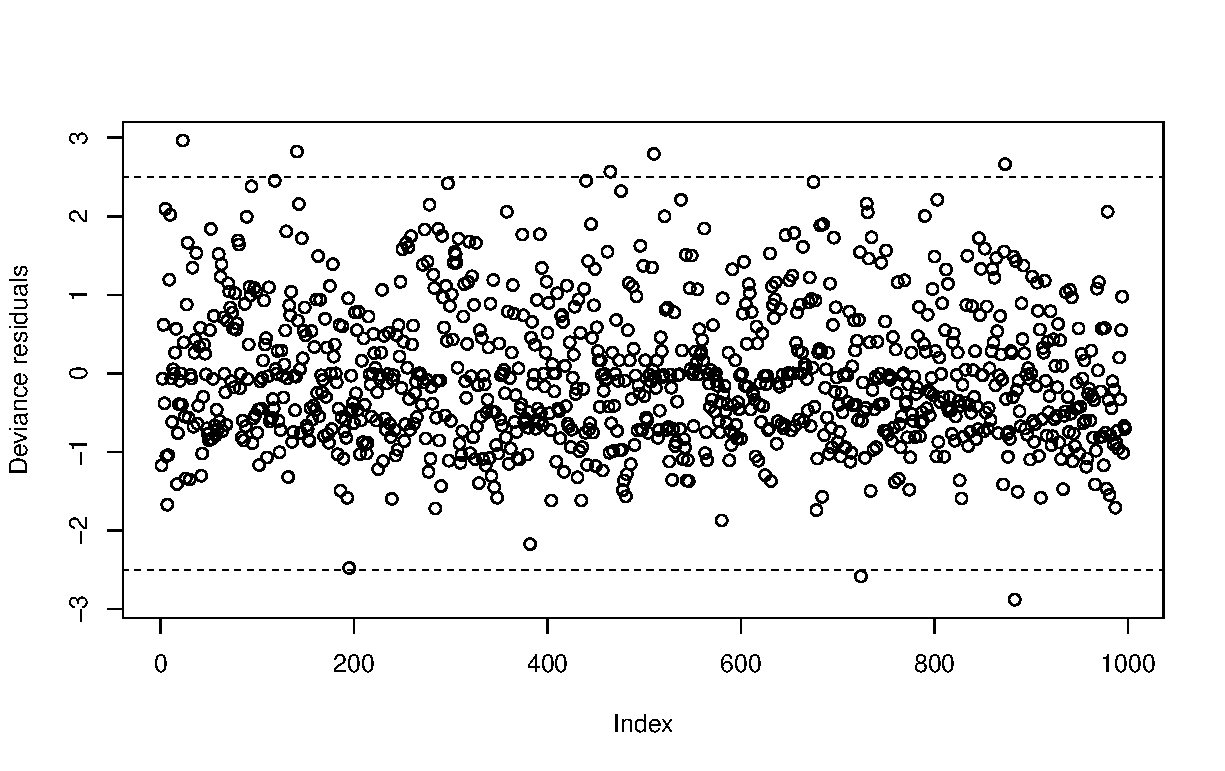
\includegraphics[width=0.7\linewidth]{fig/deviance_residuals}
\caption{}
\label{fig:devianceresiduals}
\end{figure}



%
%\subsection*{Variable selection}
%\subsection*{Logistic model}
%\subsection*{Interpretation}
%\subsection*{Apparent error rate}
%\subsection*{Error rate on test set}
%\subsection*{Linear discriminant analysis}
%\subsection*{Quadratic discriminant analysis}
%\subsection*{Comparison}


\begin{thebibliography}{9}
\bibitem{mcd} 
Rousseeuw, P. J. and Leroy, A. M. 
\textit{Robust Regression and Outlier Detection}. 
Wiley, 1987.

\bibitem{fastmcd} 
Rousseeuw, P. J. and van Driessen, K.
\textit{A fast algorithm for the minimum covariance determinant estimator.}
Technometrics 41, 212–223, 1999.

\bibitem{boxcox}
Box, G. E. P. and Cox, D. R.
\textit{An analysis of transformations (with discussion).} Journal of the Royal Statistical Society B, 26, 211–252, 1964.
\end{thebibliography}


\clearpage
\appendix

\newgeometry{left=3cm, right=3cm}
\section{Code}
\FloatBarrier
\definecolor{mygreen}{rgb}{0,0.6,0}
\definecolor{mygray}{rgb}{0.5,0.5,0.5}
\definecolor{myred}{rgb}{0.78,0,0.32}
\lstset{language=R,
        basicstyle=\scriptsize,
        breaklines=true,
        title=\lstname,
        frame=single,
        commentstyle=\color{mygreen},
        numberstyle=\tiny\color{mygray},
        keywordstyle=\color{blue},
        stringstyle=\color{myred}
}
\lstinputlisting{src/init.R}
\lstinputlisting{src/remove_RD_outliers.R}
\lstinputlisting{src/outliers_plot.R}
\lstinputlisting{src/pairs.R}
\lstinputlisting{src/transformer.R}
\lstinputlisting{src/lm.R}
\lstinputlisting{src/evaluate_lm.R}
\lstinputlisting{src/multicol.R}

\end{document}
